\subsection{Geometric interpretation of Gauss curvature}
Assume \(K_p\neq 0\).
\begin{enumerate}[(a)]
    \item \(p\in S\), \(U\) is a neighborhood of \(p\). \(N\colon
          S\to \mathbb{S}^2\) is the Gauss map.
          \begin{center}
              \tikzset{every picture/.style={line width=0.75pt}} %set default line width to 0.75pt        
              \begin{tikzpicture}[x=0.75pt,y=0.75pt,yscale=-0.9,xscale=0.9]
                  %uncomment if require: \path (0,300); %set diagram left start at 0, and has height of 300

                  %Curve Lines [id:da6642321506777753] 
                  \draw    (69,92) .. controls (109,62) and (234.4,104.
                  5) .. (274.4,74.5) ;
                  %Curve Lines [id:da5984856894036306] 
                  \draw    (38.4,193.5) .. controls (44.4,143.5) and (75.4,
                  124.5) .. (69,92) ;
                  %Curve Lines [id:da6894898997393564] 
                  \draw    (38.4,193.5) .. controls (78.4,163.5) and (203.8,
                  206) .. (243.8,176) ;
                  %Curve Lines [id:da28193586114058156] 
                  \draw    (243.8,176) .. controls (249.8,126) and (280.8,
                  107) .. (274.4,74.5) ;
                  %Shape: Circle [id:dp2732770518905623] 
                  \draw   (135.2,137.2) .. controls (135.2,123.39) and (146.
                  39,112.2) .. (160.2,112.2) .. controls (174.01,112.2) and 
                  (185.2,123.39) .. (185.2,137.2) .. controls (185.2,151.
                  01) and (174.01,162.2) .. (160.2,162.2) .. controls (146.
                  39,162.2) and (135.2,151.01) .. (135.2,137.2) -- cycle ;
                  %Shape: Circle [id:dp5729113128085532] 
                  \draw  [fill={rgb, 255:red, 0; green, 0; blue, 0 }  ,fill
                   opacity=1 ] (158,135) .. controls (158,133.78) and (158.
                   98,132.8) .. (160.2,132.8) .. controls (161.41,132.8) 
                   and (162.4,133.78) .. (162.4,135) .. controls (162.4,136.
                   22) and (161.41,137.2) .. (160.2,137.2) .. controls (158.
                   98,137.2) and (158,136.22) .. (158,135) -- cycle ;
                  %Shape: Circle [id:dp4525846429117777] 
                  \draw   (468,109.75) .. controls (468,70.4) and (499.9,38.
                  5) .. (539.25,38.5) .. controls (578.6,38.5) and (610.5,
                  70.4) .. (610.5,109.75) .. controls (610.5,149.1) and 
                  (578.6,181) .. (539.25,181) .. controls (499.9,181) and 
                  (468,149.1) .. (468,109.75) -- cycle ;
                  %Shape: Arc [id:dp8314742253507434] 
                  \draw  [draw opacity=0] (608.75,124.26) .. controls (569.
                  98,163.03) and (507.53,163.45) .. (469.27,125.18) -- (539.
                  47,54.98) -- cycle ; \draw   (608.75,124.26) .. controls 
                  (569.98,163.03) and (507.53,163.45) .. (469.27,125.18) ;
                  %Shape: Arc [id:dp9893025234051245] 
                  \draw  [draw opacity=0][dash pattern={on 0.84pt off 2.51pt}] (469.27,125.18) .. controls (508.04,86.41) and (570.49,86) .. (608.75,124.26) -- (538.55,194.46) -- cycle ; \draw  [dash pattern={on 0.84pt off 2.51pt}] (469.27,125.18) .. controls (508.04,86.41) and (570.49,86) .. (608.75,124.26) ;
                  %Shape: Arc [id:dp816831718894679] 
                  \draw  [draw opacity=0] (586.34,57.22) .. controls (555.97,71.4) and (522.37,72.11) .. (494.62,56.03) -- (557.97,-53.27) -- cycle ; \draw   (586.34,57.22) .. controls (555.97,71.4) and (522.37,72.11) .. (494.62,56.03) ;
                  %Shape: Arc [id:dp9897455191573623] 
                  \draw  [draw opacity=0][dash pattern={on 0.84pt off 2.51pt}] (494.62,56.19) .. controls (524.97,41.96) and (558.56,41.18) .. (586.34,57.22) -- (523.18,166.63) -- cycle ; \draw  [dash pattern={on 0.84pt off 2.51pt}] (494.62,56.19) .. controls (524.97,41.96) and (558.56,41.18) .. (586.34,57.22) ;
                  %Shape: Circle [id:dp6595482110117465] 
                  \draw  [fill={rgb, 255:red, 0; green, 0; blue, 0 }  ,fill opacity=1 ] (539.25,38.5) .. controls (539.25,37.28) and (540.23,36.3) .. (541.45,36.3) .. controls (542.66,36.3) and (543.65,37.28) .. (543.65,38.5) .. controls (543.65,39.72) and (542.66,40.7) .. (541.45,40.7) .. controls (540.23,40.7) and (539.25,39.72) .. (539.25,38.5) -- cycle ;
                  %Straight Lines [id:da12514301449881793] 
                  \draw    (315,131) -- (428.4,127.56) ;
                  \draw [shift={(430.4,127.5)}, rotate = 178.26] [color={rgb, 255:red, 0; green, 0; blue, 0 }  ][line width=0.75]    (10.93,-3.29) .. controls (6.95,-1.4) and (3.31,-0.3) .. (0,0) .. controls (3.31,0.3) and (6.95,1.4) .. (10.93,3.29)   ;

                  % Text Node
                  \draw (155,135.4) node [anchor=north west][inner sep=0.75pt]    {$p$};
                  % Text Node
                  \draw (195,102.4) node [anchor=north west][inner sep=0.75pt]    {$U$};
                  % Text Node
                  \draw (272,56.4) node [anchor=north west][inner sep=0.75pt]    {$S$};
                  % Text Node
                  \draw (518,13.4) node [anchor=north west][inner sep=0.75pt]    {$N( p)$};
                  % Text Node
                  \draw (624,38.4) node [anchor=north west][inner sep=0.75pt]    {$\mathbb{S}^{2}$};
                  % Text Node
                  \draw (364,102.4) node [anchor=north west][inner sep=0.75pt]    {$N$};
              \end{tikzpicture}
          \end{center}
          Let \(A\)= Area of \(U\), \(\var{A}\)= Area of \(N(U)\),
          then 
          \[
            |K(p)|=\lim_{A\to 0}\frac{\bar{A}}{A}.\tag{1}  
          \]
          \item \(p\in T_p S\)=tangent plane \(\simeq \mathbb{R}^2\). 
          Consider a circle of radius \(r\) in \(T_p S\) and a ``circle''
          of radius \(r\) on \(S\).
          \begin{center}
            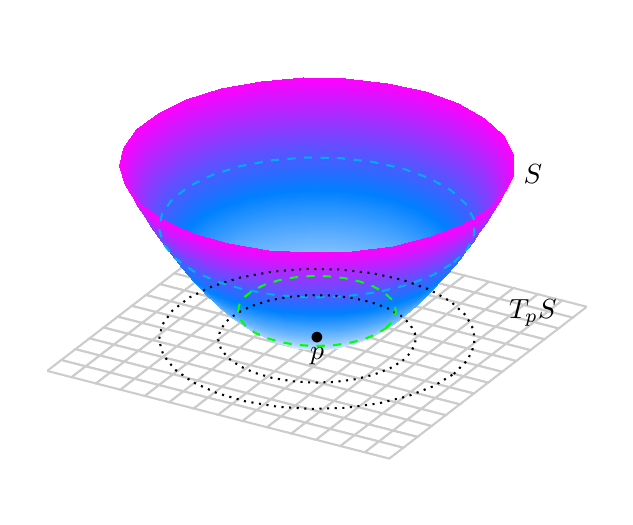
\begin{tikzpicture}
                \begin{axis}[xticklabels={,,},%不显示x坐标轴数字
                    yticklabels={,,},
                    zticklabels={,,},
                    axis line style={draw=none},%不显示坐标轴
                    tick style={draw=none},
                    colormap/cool,
                    view={30}{40}
                ]
                \addplot3 [
                    surf,
                    domain=-1:1, domain y=-1:1,
                    samples=15, samples y=15,
                ] ({x},{y},{0});
                \addplot3[
                    surf,
                    shader=interp,
                    z buffer=sort,
                    domain=0:360, domain y=0:1,
                    samples=30, samples y=30,
                    variable=\u, variable y=\v,
                    ]({v*cos(u)},{v*sin(u)},{v*v});
                    \node[text=black] at (0,0,-0.1) {\(p\)};
                    \node at (0,0,0) {\(\bullet\)};
                    \node[text=black] at (0.8,0.8,0) {\(T_p S\)};
                    \node[text=black] at (0.8,0.8,0.8) {\(S\)};
                \addplot3 [
                    black,
                    dotted,
                    domain=0:360,
                    samples=30,
                    samples y=1%防止曲线闭合
                ]({0.8*cos(x)},{0.8*sin(x)},0);
                \addplot3 [
                    cyan,
                    dashed,
                    domain=0:360,
                    samples=30,
                    samples y=1%防止曲线闭合
                ]({0.8*cos(x)},{0.8*sin(x)},{0.64});
                \addplot3 [
                    black,
                    dotted,
                    domain=0:360,
                    samples=30,
                    samples y=1%防止曲线闭合
                ]({0.5*cos(x)},{0.5*sin(x)},0);
                \addplot3 [
                    green,
                    dashed,
                    domain=0:360,
                    samples=30,
                    samples y=1%防止曲线闭合
                ]({0.4*cos(x)},{0.4*sin(x)},{0.16});
                \end{axis} 
            \end{tikzpicture}
          \end{center}
          Then
          \[\label{geometric meaning curvature 2}
            K(p)=\lim_{r\to 0}3\frac{2\pi r-c(r)}{\pi r^3},\tag{2}  
          \]
          where \(c(r)\)= circumference of the circle of radius \(r\)
          on \(S\).
          \item Consider a disk around \(p\) of radius \(r\) in \(T_p S\). 
          Also consider a ``disk'' around \(p\) of radius \(r\) on 
          \(S\).
          \[\label{geometric meaning curvature 3}
            K(p)=\lim_{r\to 0} 12\frac{\pi r^2-A(r)}{\pi r^4},\tag{3}
          \]
          where \(A(r)\)= Area of disk on \(S\).
\end{enumerate}
\begin{remark}
    From expression of \cref{geometric meaning curvature 2} 
    and \cref{geometric meaning curvature 3}, one can prove 
    them by considering the Taylor's expansion of \(c(r)\)
    and \(A(r)\). The proof of these two facts will be postponed
     after we step into intrinsic geometry.(Need Taylor's expansion
      of metric tensor)
\end{remark}
\begin{proof}
    Let \(F(u,v)\) be the local parametrization on \(U\).
    \[
        \Rightarrow Area(U)=\iint_{F^{-1}(U)}\left|
            F_u\wedge F_v
        \right| \dd u\dd v,
    \]
    then \(T_{N(p)}N(U)=\Span\{N_u,N_v\}\),
    \[
        \bar{A}=\iint_{F^{-1}(U)} \left|N_u\wedge N_v\right|\dd u
        \dd v.
    \]
    \underline{Recall}: \(dN\begin{pmatrix}
        F_u\\
        F_v
    \end{pmatrix}=\begin{pmatrix}
        N_u\\N_v
    \end{pmatrix}=A\begin{pmatrix}
        F_u\\
        F_v
    \end{pmatrix}\), where \(A\) is the Weingarten matrix.
    \[
        \Rightarrow \left|
            N_u \wedge N_v
        \right|=\left|\det A\right|\left|
            F_u\wedge F_v
        \right|=|K|\left|
            F_u\wedge F_v
        \right|.
    \]
    \begin{align*}
        \frac{\bar{A}}{A}&=\frac{\iint |K|\left|
            F_u\wedge F_v
        \right|\dd u \dd v}{\iint \left|
            F_u\wedge F_v
        \right|\dd u\dd v}\\
        &=\frac{|K(q)|\left|
            F_u\wedge F_v
        \right|(q)Area(F^{-1}(U))}{\left|
            F_u\wedge F_v
        \right|(\bar{q})Area(F^{-1}(U))}\quad (\text{Middle value theorem}).
    \end{align*}
    As \(A\to 0\), \(q\to p\), \(\bar{q}\to p\),
    \[\Rightarrow |K(p)|=\lim_{A\to 0}\frac{\bar{A}}{A}.\]
\end{proof}
\section{More Examples}
\begin{exercise}
    Graph \(z=h(x,y)\)= \(S\). 
\end{exercise}
(\underline{Recall}: For a regular surface, by the implicit (inverse) 
function theorem, it can be written as a graph locally.)

In the HW 8, you may have computed 
\[
    I=\left(1+h_x^2\right)\dd x^2+2h_x h_y\dd x\dd y+(1+h_y^2)\dd y^2
\]
\[
    \II =\frac{h_{xx}}{\sqrt{1+\left|\nabla h\right|_{\mathbb{R}^2}^2}}
    \dd x^2 +2 \frac{h_{x}h_y}{\sqrt{1+\left|\nabla h
    \right|^2}}\dd x\dd y+\frac{h_{yy}}{\sqrt{1+\left|
        \nabla h\right|^2}}\dd y^2.
\]
\[
N=\frac{\left(-h_x,-h_y,1\right)}{\sqrt{1+\left|
    \nabla h\right|^2}}.    
\]
\[
    K=\frac{h_{xx}h_{yy}-h_{xy}^2}{\left(1+\left|
        \nabla h\right|^2\right)^2}=\frac{\det \nabla^2h}{\left(1+\left|
            \nabla h\right|^2\right)^2}.
\]
\[
    2H=\frac{(1+h_x^2)h_{yy}-2 h_x h_y h_{xy}+(1+h_y^2)h_{xx}}{
        \left(1+\left|
            \nabla h\right|^2\right)^{\frac{3}{2}}
    }    .
    \footnotemark
\]
\footnotetext{A basic observation one should make is how \(K\) and
\(H\) depend on the \engordnumber{2} derivative of \(h\).}
Note that the last term equals \[
    \mathrm{div}_{\mathbb{R}^2}\left(\frac{\nabla h}{
        \sqrt{1+\left|
            \nabla h\right|^2}
    }\right)
    =
    \sum_{i,j=1}^2 L^{ij}\left(\nabla f\right)\nabla_i\nabla_j h,
\]
where \[
    L^{ij}\left(\nabla f\right)=\frac{1}{\sqrt{1+\left|
        \nabla h\right|^2}}\left(\delta_{ij}-
        \frac{\nabla_i h\nabla_j h}{1+\left|
            \nabla h\right|^2}\right)    .
\]
Let \(p\in S\), and assume \(p\) is the origin in \(\mathbb{R}^3\),
 and \(N\) agrees with the unit normal of \(z\)-axis
 \[
    h_x=h_y=0\text{ at p}.   
 \]
 \[
    e=h_{xx}(0,0), f=h_{xy}(0,0), g=h_{yy}(0,0).   
 \]
 Hessian of \(h\) at \(p\) is 
 \[
    \begin{pmatrix}
        h_{xx}(0,0)& h_{xy}(0,0)\\
        h_{yx}(0,0)&h_{yy}(0,0)
    \end{pmatrix} .  
 \]
 Hence, at \(p\)
 \[
    \II=\mathrm{Hess}~h.   
 \]
 Moreover, at \(p\)
 \[
    \partial H=\delta h.
 \]
 As an application, we give a geometric interpretation of the Dupin
 indicatrix.
 \underline{Claim}: If \(p\in S\) is not a planar point, consider the 
 intersection of a plane parallel to \(T_p S\) with \(S\), and the plane
  is close enough to \(T_p S\), then the obtained curve is approximated
   by the Dupin indicatrix.
\begin{proof}
    Since we only care about local behavior at \(p\), W.L.O.G assume
     near \(p\), the surface is parametrized by the graph \(z=h(x,y)\),
     such that \(p\) is the origin and \(z\)-axis is the normal direction 
      and \(x\)-axis, \(y\)-axis are principal directions.
      Let the intersection curve be \(h(x,y)=\epsilon\), for sufficiently
      small \(\epsilon\). Consider the Tayler's expansion of 
      \(h(x,y)\) at \(p\)
      \begin{align*}
        h(x,y)=&h(0,0)+h_x(0,0)x+h_y(0,0)y\\
        &+\frac{1}{2}\left(
            h_{xx}(0,0)x^2+\underbrace{2h_{xy}(0,0)}_{
                =0\text{(principal direction)}
            }xy+h_yy(0,0)y^2
        \right)\\
        &+\text{Remainder}\\
        =&\frac{1}{2}\begin{pmatrix}
            x&y
        \end{pmatrix}
        \begin{pmatrix}
            h_{xx}(0,0)&0\\
            0&h_{yy}(0,0)
        \end{pmatrix}
        \begin{pmatrix}
            x\\
            y
        \end{pmatrix}+\text{Remainder},
      \end{align*}
\end{proof}
where 
\[
    \lim_{(x,y)\to (0,0)}    \frac{\text{Remainder}}{x^2+y^2}=0.
\]
Hence, the intersection curve is given by 
\[
    \frac{1}{2}\left(h_{xx}(0,0)x^2+h_{yy}(0,0)y^2\right)+R=\epsilon.    
\]
Note: in the \engordnumber{2} fundamental form\(II\) \(f=0\), 
and in the  \engordnumber{1} fundamental form \(I\) \(F=0\),
then at \(p\) one has 
\[
    \begin{cases}
        k_1=\frac{e}{E}=h_{xx}(0,0)\\
        k_2=\frac{g}{G}=h_{yy}(0,0)
    \end{cases}    
\]
using \(k_i=H\pm\sqrt{H^2-K}\). Then, \(k_1x^2+k_2y^2=2\epsilon\)
can be viewed as the \engordnumber{1} order approximation of the 
intersection curve. Renormalized it, then 
\[k_1 \bar{x}^2+k_2\bar{y}^2=1.\]
is just the Dupin indicatrix.
\begin{exercise}
    Surface of revolution.
\end{exercise}
Let \(\alpha(s)=\varphi(s),0,\psi(s)\) be a regular curve, with \(\varphi
(s)>0\) and \(s\in(a,b)\) is the arclength parametrization.
\(\Rightarrow \left(\varphi'(s)\right)^2+\left(\psi'(s)\right)^2=1\)
\(\Rightarrow \vphi'\vphi'' +\psi'\psi''=0\).
Rotate it about \(z\)-axis
\[
    \Rightarrow \alpha(\theta,s)=\left(\varphi(s)\cos\theta
    ,\varphi(s)\sin \theta,\psi(s)\right),\, 0<\theta<2\pi.
\]
\begin{align*}
    I=&\dd s^2+\varphi(s)^2\dd \theta^2\\
    \II=&\left(\psi'\vphi''-\psi''\vphi'\right)\dd s^2
    -\vphi\psi'\dd\theta^2.
\end{align*}
\(\because F=f=0\), \(\therefore\) \(s\)-curve and \(\theta\)-curve 
are curvature lines.
\[
    K=\frac{e}{E}\frac{g}{G}=-\frac{\varphi''}{\varphi},\;
    H=\frac{1}{2}\left(\frac{e}{E}+\frac{g}{G}\right)    .
\]
Since principal curvatures satisfy \(\lambda^2-2\lambda H+K=0\).
\[
    \Rightarrow \lambda_1    =\frac{e}{E}=-\frac{\vphi''}{\vphi},
    \;\lambda_2=\frac{g}{G}=\psi'\vphi''-\psi''\vphi'.
\]
The mean curvature is 
\[
    H=\frac{1}{2}\frac{-\psi'+\vphi\left(\psi'\vphi''-
    \psi''\vphi'\right)}{\vphi}.    
\]
\begin{question}[Homework]
    \begin{enumerate}[(1)]
        \item Assume \(K=1\), \(\lim_{s\to 0^+}\alpha(s)=(0,0,1)\),
         \(\alpha(\frac{\pi}{2})=(1,0,0)\),\(s\in (0,\pi)\). 
         Describe the surface and determine the \engordnumber{1}
         fundamental form (\(\dd s^2+\sin^2 s\dd \theta^2\)).
         \item Assume \(K=0\), \(\lim_{s\to 0^+}\alpha(s)=(0,0,1)\),
          \(\alpha(1)=(\frac{\sqrt{2}}{2},0,\sqrt{2}{2})\), 
          \(s\in (0,\infty)\), answer the same question as in (1)
          (\(\dd s^2+\frac{1}{2}s^2\dd \theta^2\)).
          \item Assume \(H=0\), \(\alpha(0)=(1,0,0)\), \(\alpha(1)
          =(\sqrt{2},0,\arcsin(1))\), \(s>0\), answer the question in 
          (1). (\(\alpha(s)=\left(\sqrt{1+s^2},0,\arcsin s\right)\),
           \(I=\dd s^2+(1+s^2)^2\dd \theta^2\sim \text{Catenoid}\)).
    \end{enumerate}
\end{question}

\begin{exercise}[Ruled surface]
    A line passing through a point \(\alpha_0\in\mathbb{R}^3\) 
    with direction \(v\in \mathbb{R}^3\) can be written as 
    \[
        \ell(t)=\alpha_0 + t v.    
    \]
    Now we let \(\alpha_0,v\) are two vector-valued functions,
    \ie\ \(\alpha(s),v(s)\), then the collection of lines form 
    a surface 
    \[
        R(s,t)=\alpha(s)+t v(s).    
    \]
Surfaces with such parametrization is called the ruled surfaces, 
where \(\alpha(s)\) is called the base curve of \(S\) and 
\(v(s)\) is called the director curve.
\end{exercise}
\begin{remark}
    Ruled surface may contain singular points.
\end{remark}
\begin{example}
    \(R(s,t)=\alpha(s)+t e_3\). \(\alpha(s)\) is the circle on \(x-y\)
    plane, \(e_3=(0,0,1)\). (\(x^2+y^2=1\)) 
    \begin{center}
            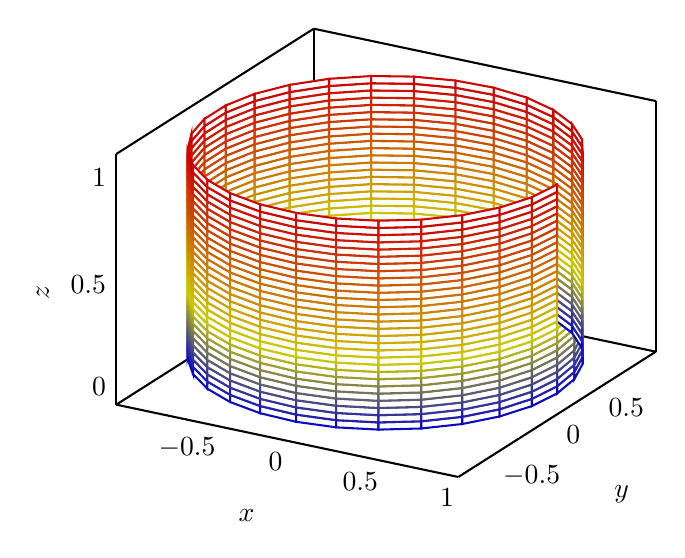
\begin{tikzpicture}
                \begin{axis}[
                    %xticklabels={,,},%不显示x坐标轴数字
                    %yticklabels={,,},
                    %zticklabels={,,},
                    %axis line style={draw=none},%不显示坐标轴
                    tick style={draw=none},
                    view={30}{30},
                    xlabel=\(x\),
                    ylabel=\(y\),
                    zlabel=\(z\)
                ]
                \addplot3 [
                    surf,
                    fill=white,
                    domain=0:1, domain y=0:360,
                    samples=30, samples y=30,
                ] ({cos(y)},{sin(y)},{x});
                \end{axis}
            \end{tikzpicture}
        \end{center}
\end{example}
\begin{example}\label{a ruled surface}
    \(R(s,t)=\alpha(s)+t\left(\alpha'(s)+e_3\right)\), where \(\alpha(s)\)
     and \(e_3\) are the same as before.
    \begin{center}
        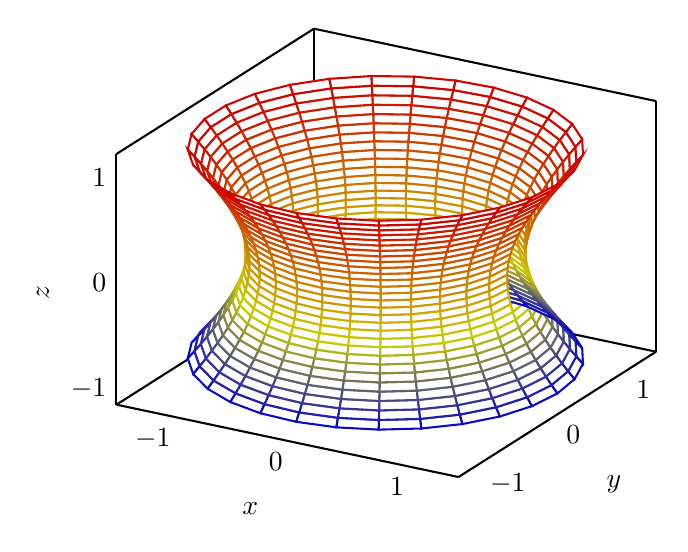
\begin{tikzpicture}
            \begin{axis}[
                %xticklabels={,,},%不显示x坐标轴数字
                %yticklabels={,,},
                %zticklabels={,,},
                %axis line style={draw=none},%不显示坐标轴
                tick style={draw=none},
               % colormap/cool,
                view={30}{30},
                xlabel=\(x\),
                ylabel=\(y\),
                zlabel=\(z\)
            ]
            \addplot3 [
                surf,
                fill=white,
                domain=-1:1, domain y=0:360,
                samples=30, samples y=30,
            ] ({sqrt(x*x+1)*cos(y)},{sqrt(x*x+1)*sin(y)},{x});
            \end{axis}
        \end{tikzpicture}
    \end{center}
\end{example}
\begin{example}
    \(R(s,t)=0+t\left(u(s)+e_3\right)\), where \(u(s)=\left(
        \cos\theta,\sin\theta,0
    \right)\)
    \begin{center}
        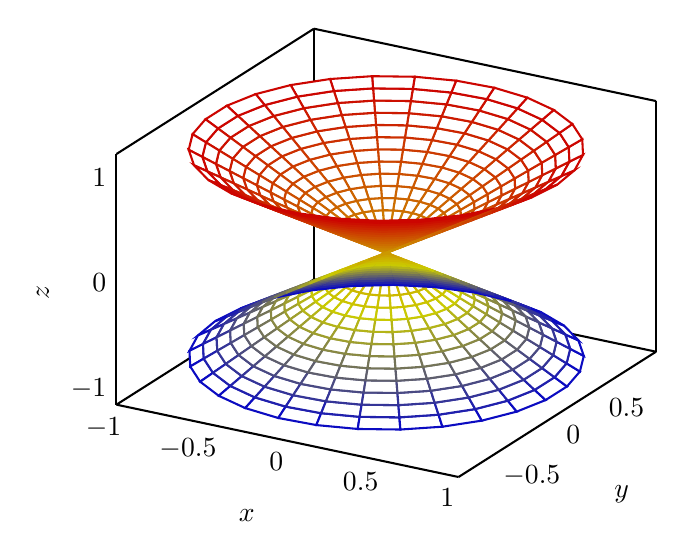
\begin{tikzpicture}
            \begin{axis}[
                %xticklabels={,,},%不显示x坐标轴数字
                %yticklabels={,,},
                %zticklabels={,,},
                %axis line style={draw=none},%不显示坐标轴
                tick style={draw=none},
                view={30}{30},
                xlabel=\(x\),
                ylabel=\(y\),
                zlabel=\(z\)
            ]
            \addplot3 [
                surf,
                fill=white,
                domain=-1:1, domain y=0:360,
                samples=30, samples y=30,
            ] ({x*cos(y)},{x*sin(y)},{x});
            \end{axis}
        \end{tikzpicture}
    \end{center}
\end{example}
In the following discussion, we assume the ruled surface \(S\)
\[
    R(s,t)=\alpha(s)+t v(s),~|v(s)|=1,~v'(s)\neq 0\forall s.    
\]
Direct computation shows:
\begin{align*}
    I=&\left|\alpha_s+t v_s\right|^2\dd s^2+2\left\langle
        \alpha_s,v
    \right\rangle \dd s\dd t
    +\dd t^2\\
    N=&\frac{\alpha_s\wedge v+t v_s \wedge v}{
        \left|\alpha_s\wedge v+t v_s \wedge v\right|
    }\\
    \II=&e\dd s^2+2f \dd s \dd t .
\end{align*}
Hence,
\[
    K=-\frac{f^2}{\det I}\le 0.    
\]
Note that 
\begin{align*}
    f&=\left\langle R_{st},N\right\rangle\\
    &=v_s\vdot \frac{\alpha_s\wedge v+t v_s \wedge v}{
        \left|\alpha_s\wedge v+t v_s \wedge v\right|
    }\\
    &=\frac{\left(v_s,\alpha_s,v\right)}{\left|R_s\wedge R_t\right|}.
\end{align*}
\begin{definition}
    \(S\) is called developable on ``flat'' surface if \(\left(
        v_s,v,\alpha_s
    \right)\equiv 0\). In this case \(K=0\).
\end{definition}
\begin{remark}
    Physically, a developable surface can be flattened onto a plane 
    without ``stretching'' or ``compressing'', but allowing unfolding
    or cutting along a line. Later, we'll see on page 414, section 5-8
    in Do Carmo: If on a developable surface \(S\), all lines can be 
    extended on both sides, the surface can only be a plane 
    or a cylinder.
\end{remark}
\begin{remark}
    On a noncylindrical ruled surface \(S\), \ie\ 
    \[R(s,t)=\alpha(s)+t v(s),v'(s)\neq 0\forall s,\]
    one can choose a spherical base curve \(\beta(s)\) such
    that 
    \[
        R(s,t)=\beta(s)+t v(s),    
    \]
    where \(\left\langle\beta'(s)+v'(s)\right\rangle=0\),
     such curve is called the line of striction. Points on the line
      of striction is called the central points of the ruled surface.
\end{remark}
\begin{example}
    In \cref{a ruled surface}, \(\alpha(s)\) is the line of striction.
\end{example}
\begin{exercise}
    Find the line of restriction (\(\beta(s)-\alpha(s)
    -\frac{\left\langle\alpha',v'\right\rangle}{|v'|^2}v\)).
    Then \(R(s,u)=\beta(s)+u v(s)\).

    Hence if we let \(\lambda=\frac{(\beta',v,v')}{|v'|^2}\), then 
    \(K=-\frac{\lambda^2}{\left(\lambda^2+u^2\right)^2}\).
\end{exercise}
\begin{exercise}[Homework]
    Prove that there are no closed smooth minimal surface in 
    \(\mathbb{R}^2\).
\end{exercise}
\begin{proof}
    On a closed surface, there must exist an elliptic point, at which 
    \(k>0\), this contradicts to minimal surface.
\end{proof}
\begin{theorem}
    \begin{enumerate}[(1)]
        \item If a surface of revolution \(M\) is minimal, then 
        \(M\) is contained in either a plane or a catenoid.
        \item If a ruled surface \(M\) is minimal, then \(M\) is 
        contained in either a plane or a helicoid.
    \end{enumerate}
\end{theorem}
\begin{proof}
    See homework.
\end{proof}
\section{Isometries between surfaces}
From this lecture on, we'll study the intrinsic geometry of a regular 
surface. More precisely, we'll see how the \engordnumber{1} fundamental
form determines the geometry.
\begin{itemize}
    \item \(S_1,S_2\) are regular Surfaces, \(f\colon S_1\to S_2\).
\end{itemize}
\begin{enumerate}[(1)]
    \item \(f\) is isomorphism (1-1 and onto) 
    (of sets)\(\Leftrightarrow \)
    \(S_1\) and \(S_2\) are identified as sets.
    \item \(f\) is homeomorphism (\(f\) is an isomorphism + \(f\)
    and \(f^{-1}\) continuous)\(Leftrightarrow\) \(S_1\) and \(S_2\)
    are identified as topological spaces.
    \item \(f\) is diffeomorphism (\(f\) is a homeomorphism+
    \(f,f^{-1}\) are smooth) \(\Leftrightarrow\) \(S_1\) and \(S_2\)
    are identified with considering smooth structures on them.
    \item \(f\) is isometry 
    
    \(\Leftrightarrow\) \(f\)
    is a diffeomorphism and \(f\) preserves the arclength, 
    area, angles,\(\ldots\)(everything defined by the 
    \engordnumber{1} fundamental form).
\end{enumerate}
\begin{definition}[Isometry]
    \(\vphi\colon S_1\to S_2\) is a diffeomorphism between regular 
    surfaces. If \(\forall p\in S_1\), \(v_1,v_2\in T_p S\)
    \[
        \left\langle v_1,v_2\right\rangle_p=
        \left\langle d\vphi_p(v_1),d\vphi_p(v_2)\right\rangle,
        \tag{1}\label{definition of isometry}
    \]
    which is equivalent to saying that \(\vphi\) preserves the 
    \engordnumber{1} fundamental form, then we say \(\vphi\) is 
    an isometry.
\end{definition}
\begin{definition}[Local isometry]
    \(\vphi\colon S_1\to S_2\) is called a local isometry, if 
    \(\forall p\in S_1\), \(\exists\) a neighborhood \(U\) of 
    \(p\) such that \(\vphi|_U\) is an isometry.
\end{definition}
\begin{example}
    Catenoid and helicoid are only locally isometric to each other but not 
    global isometric. In fact the helicoid is simply connected, but 
    the catenoid is not (since it comes from revolution).
\end{example}
\begin{remark}
    Isometry implies local isometry, however the converse is false.
\end{remark}
\begin{example}
    \(\left(\mathbb{R}^2,\dd x^2 +\dd y^2\right)\) and the cylinder 
    \((\cos u,\sin u,v), \dd u^2+\dd v^2\) are only local isometric
     to each other, but not ``globally'' isometric.

    (The local isometry map is just the local parametrization
    of cylinder:
    \[
        \vphi\colon (u,v,0)\to (\cos u,\sin u,v).    
    \]
    Clearly, \(\mathbb{R}^2\) and the cylinder are not diffeomorphic
    to each other, since the cylinder has a non-shrinkable loop.)
\end{example}
\begin{exercise}
    The condition in \cref{definition of isometry} is equivalent to 
    \[
        \forall w\in T_p S, \quad |w|_p=\left|d \vphi_p(w)
        \right|_{\varphi(p)}.\tag{2}\label{second definition of isometry}
    \]
\end{exercise}
\begin{proof}
    \cref{definition of isometry} \(\Rightarrow\)
     \cref{second definition of isometry}, obviously.

     \cref{second definition of isometry}
     \(\Rightarrow\) \cref{definition of isometry}, 
     let  \(w=v_1+v_2\), then 
     \[
        |w|_p^2=\left|d \vphi_p(w)
        \right|_{\varphi(p)}^2,~
        |v_1|_p^2=\left|d \vphi_p(v_1)
        \right|_{\varphi(p)}^2,~ 
        |v_2|_p^2=\left|d \vphi_p(v_2)
        \right|_{\varphi(p)}^2
     \]
     \[\Rightarrow
        \left\langle v_1,v_2\right\rangle_p=
        \left\langle d\vphi_p(v_1),d\vphi_p(v_2)\right\rangle.
     \]
\end{proof}
\begin{remark}
    If \(\vphi\colon S_1\to S_2\) is a local isometry.
    \(\forall p\in S_1\), let \(U\) be a coordinate patch of 
    \(p\) and \(\vphi|_U\colon U\to \vphi(U)\) is a diffeomorphism 
    given by 
    \[
        \vphi(u,v)=\left(\tilde{u},\tilde{v}\right).    
    \]
    \[
        I_1=\begin{pmatrix}
            \dd u& \dd v
        \end{pmatrix}
        \begin{pmatrix}
            E&F\\
            F&G
        \end{pmatrix}
        \begin{pmatrix}
            \dd u\\
            \dd v
        \end{pmatrix}
    \]
    \[
        I_2=\begin{pmatrix}
            \dd \tilde{u}& \dd \tilde{v}
        \end{pmatrix}
        \begin{pmatrix}
            \tilde{E}&\tilde{F}\\
            \tilde{F}&\tilde{G}
        \end{pmatrix}
        \begin{pmatrix}
            \dd \tilde{u}\\
            \dd \tilde{v}
        \end{pmatrix}.
    \]
    Note 
    \[
        \begin{pmatrix}
            \dd \tilde{u}\\
            \dd \tilde{v}
        \end{pmatrix}
        =
        \pdv{(\tilde{u},\tilde{v})}{(u,v)}
        \begin{pmatrix}
            \dd u\\
            \dd v
        \end{pmatrix}
        =
        J_\vphi 
        \begin{pmatrix}
            \dd u\\
            \dd v
        \end{pmatrix}    
    \]
    \[
        \Rightarrow 
        \begin{pmatrix}
            E&F\\
            F&G
        \end{pmatrix}=
        J_\vphi^\top \begin{pmatrix}
            \tilde{E}&\tilde{F}\\
            \tilde{F}&\tilde{G}
        \end{pmatrix} J_\vphi. 
    \]
\end{remark}